\documentclass[border=6pt]{standalone}
\usepackage{tikz}
\begin{document}
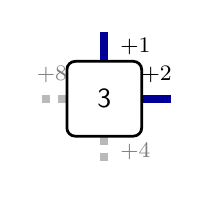
\begin{tikzpicture}[font=\sffamily,
    tile/.style={draw, rounded corners=3pt, fill=white, minimum size=0.95cm,
                 line width=1pt, inner sep=0pt},
    open/.style={line width=3pt, draw=blue!60!black},
    closed/.style={line width=3pt, draw=gray!55, dashed},
    bitlab/.style={font=\sffamily\footnotesize\itshape}]
  % one junction with openings up (1) and right (2): g = 1 + 2 = 3
  \draw[open]   (0, 0.48) -- (0, 0.85) node[bitlab, midway, right=1pt] {$+1$};
  \draw[open]   (0.48, 0) -- (0.85, 0) node[bitlab, midway, above=1pt] {$+2$};
  \draw[closed] (0,-0.48) -- (0,-0.85) node[bitlab, midway, right=1pt, gray] {$+4$};
  \draw[closed] (-0.48,0) -- (-0.85,0) node[bitlab, midway, above=1pt, gray] {$+8$};
  \node[tile] at (0,0) {3};
\end{tikzpicture}
\end{document}
